\documentclass{beamer}
\usepackage[utf8]{inputenc}
\usepackage[pdf,tmpdir]{graphviz}
\usepackage{graphicx}
\usepackage{svg}
\usepackage[dvipsnames]{xcolor}
\usepackage{mathrsfs}
\usepackage{bbold}
\usepackage[export]{adjustbox}
\usepackage{stmaryrd}

\setbeamertemplate{navigation symbols}{}
\usefonttheme[onlymath]{serif}
\graphicspath{{./assets/}}

\definecolor{msg-color}{RGB}{77,0,0}
\definecolor{keyword}{RGB}{8,0,153}

\newcommand{\msgtag}[1]{\texttt{\textcolor{msg-color}{#1}}}
\newcommand{\msgstore}[2]{\msgtag{#1}[\overline{#2}]}
\newcommand{\msgreceive}[2]{\msgtag{#1}(\overline{#2})}
\newcommand{\done}{\texttt{\textcolor{keyword}{done}}}
\newcommand{\free}[1]{\texttt{\textcolor{keyword}{free}}\hspace{0.25em}#1}
\newcommand{\fail}[1]{\texttt{\textcolor{keyword}{fail}}\hspace{0.25em}#1}
\newcommand{\parbar}{\kern3pt\rule[-3pt]{0.8pt}{0.9\baselineskip}\kern3pt}

\title{Mailbox Types for Unordered Interactions\footnote{\tiny{Ugo de'Liguoro, Luca Padovani (2018). https://arxiv.org/abs/1801.04167}}}
\titlegraphic{\includesvg[scale=0.2]{assets/mailbox.svg}}
\author{Presentación por Jonathan Bekenstein}
\institute{Materia optativa sobre Tipos Comportamentales y Contratos}
\date{2024}

\begin{document}

\frame{\titlepage}

\begin{frame}{Introducción}
    Buscamos modelar protocolos de comunicación en diferentes topologías de procesos concurrentes. La comunicación es \textbf{multi-party} y sucede mediante el uso de \textbf{mailboxes} no ordenados, en donde:
    \begin{itemize}
        \item procesos pueden escribir mensajes identificados por un \emph{tag} con argumentos opcionales,
        \item procesos pueden consumir (leer) los mensajes en un orden arbitrario (\emph{out-of-order} o \emph{selective processing}).
    \end{itemize}

    \center
    \vspace{-1em}
    \digraph[scale=0.4]{intro}{
        graph [rankdir=LR, pad=0.1]
        node [shape=circle, fontname="Latin Modern Mono"]
        mailbox [shape=box]
        P1 -> mailbox
        P2 -> mailbox
        P3 -> mailbox
        mailbox -> Q
    }
    \vspace{-1em}

    Procesos bien tipados respetan el protocolo y no tienen deadlocks.
\end{frame}

\begin{frame}{Mailbox calculus}{Sintaxis: gramática}
    \begin{figure}[H]
        \centering
        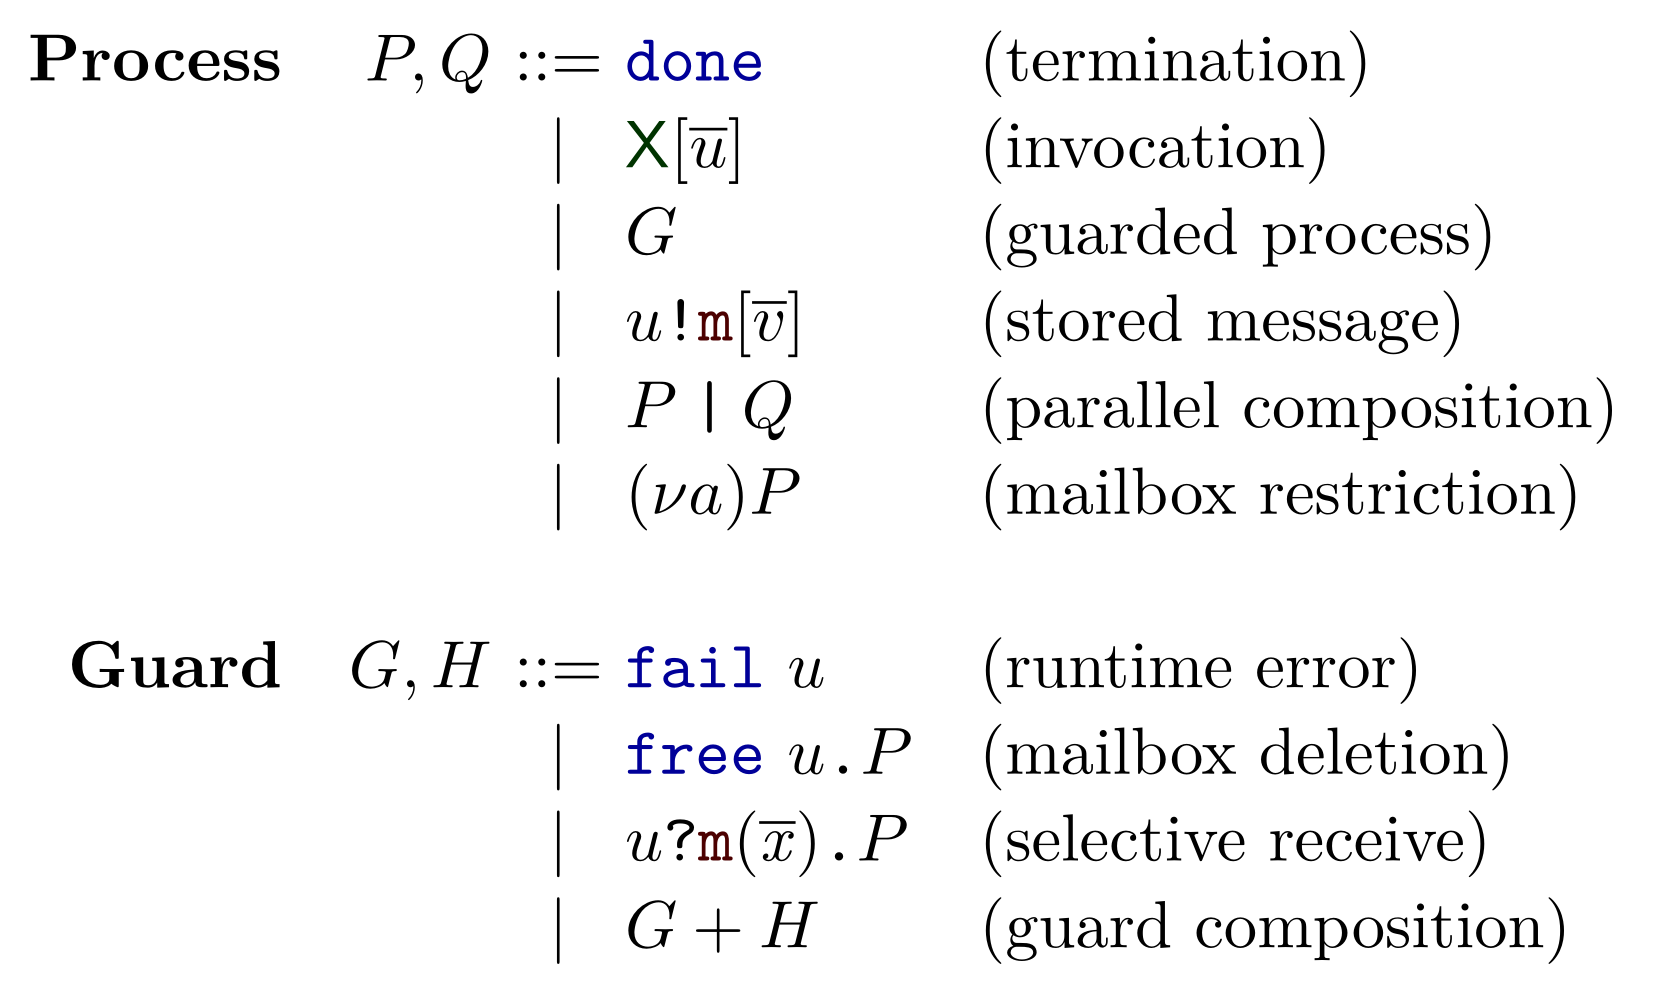
\includegraphics[width=0.8\textwidth]{syntax}
    \end{figure}

    \footnotesize{$\overline{u}$ denota la secuencia $u_1, \dots, u_n$}
\end{frame}

\begin{frame}{Mailbox calculus}{Sintaxis: mensajes}
    \begin{block}{Enviar mensajes}
        $u!\msgstore{m}{v}$
        \\ Guarda un mensaje identificado con el tag $\msgtag{m}$ y argumentos $\overline{v}$ en el mailbox $u$.
    \end{block}

    \begin{block}{Recibir mensajes}
        $u?\msgreceive{m}{x}.P$ \\ Consume selectivamente el mensaje con tag $\msgtag{m}$ del mailbox $u$ y continúa con $P$ reemplazando $\overline{x}$ por los argumentos del mensaje.
    \end{block}
\end{frame}

\begin{frame}{Mailbox calculus}{Sintaxis: procesos}
    \begin{block}{Invocación}
        $\text{X}[\overline{u}]$ representa la invocación de un proceso llamado $\text{X}$ con parámetros $\overline{u}$. Asumimos que existe una definición global de procesos de la forma $\text{X}(\overline{x}) \triangleq P$.
    \end{block}

    \begin{block}{Paralelo y restricción}
        $P \parbar Q$ denota la composición paralela de procesos, y $(\nu a) P$ representa un mailbox $a$ restringido al scope de $P$.
    \end{block}

    \begin{block}{Terminación}
        Un proceso $\done$ representa un proceso terminado y que no realiza ninguna otra acción.
    \end{block}
\end{frame}

\begin{frame}{Mailbox calculus}{Sintaxis: guardas}
    \begin{block}{Guardas}
        Las guardas $G$ y la composición de guardas $G+H$ nos permite modelar distintas ``ramas'' de ejecución en función del mensaje consumido del mailbox. Luego se usa exclusivamente la continuación de la guarda que consumió el mensaje.
    \end{block}

    \begin{block}{Errores}
        $\fail{u}$ permite modelar un runtime error al recibir un mensaje inesperado.
    \end{block}

    \begin{block}{Eliminar mailbox}
        $\free{u}.P$ permite eliminar el mailbox $u$ si ya no se va a utilizar y continuar la ejecución con $P$.
    \end{block}
\end{frame}

\begin{frame}{Mailbox calculus}{Semántica operacional}
    \begin{block}{Reglas de reducción}
        \begin{figure}[H]
            \centering
            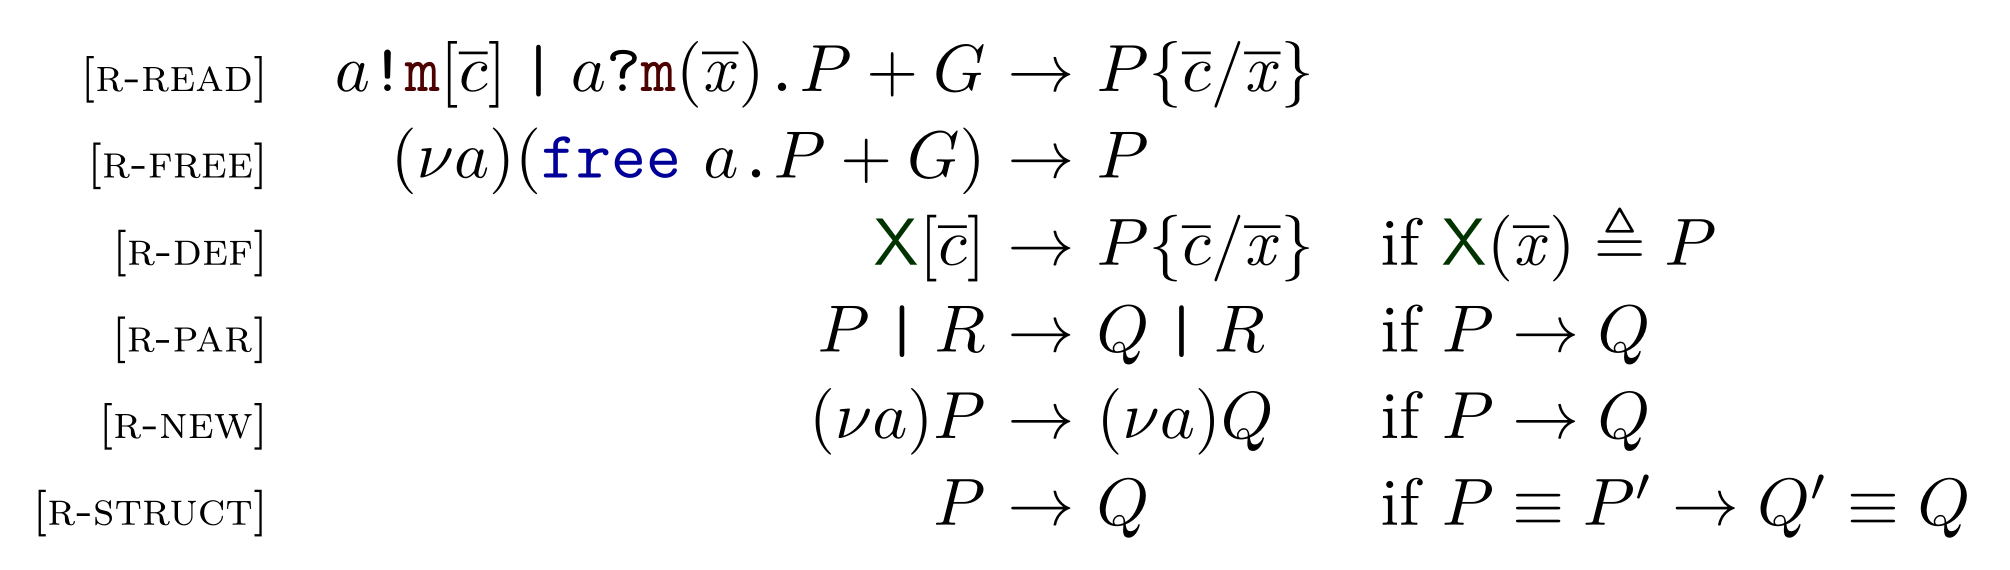
\includegraphics[width=0.9\textwidth]{reduction-rules}
        \end{figure}
    \end{block}

    \begin{block}{Relación de congruencia estructural}
        \begin{figure}[H]
            \centering
            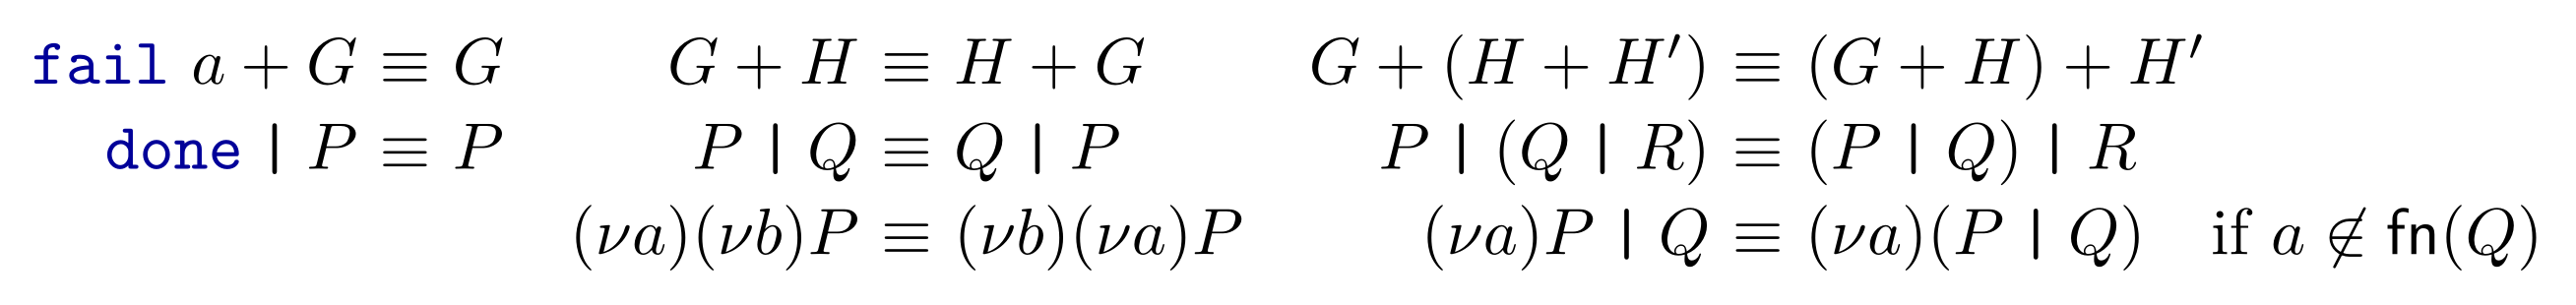
\includegraphics[width=0.9\textwidth]{structural-congruence}
        \end{figure}
    \end{block}
\end{frame}

\begin{frame}{Ejemplo 1: Lock}
    \begin{figure}[H]
        \centering
        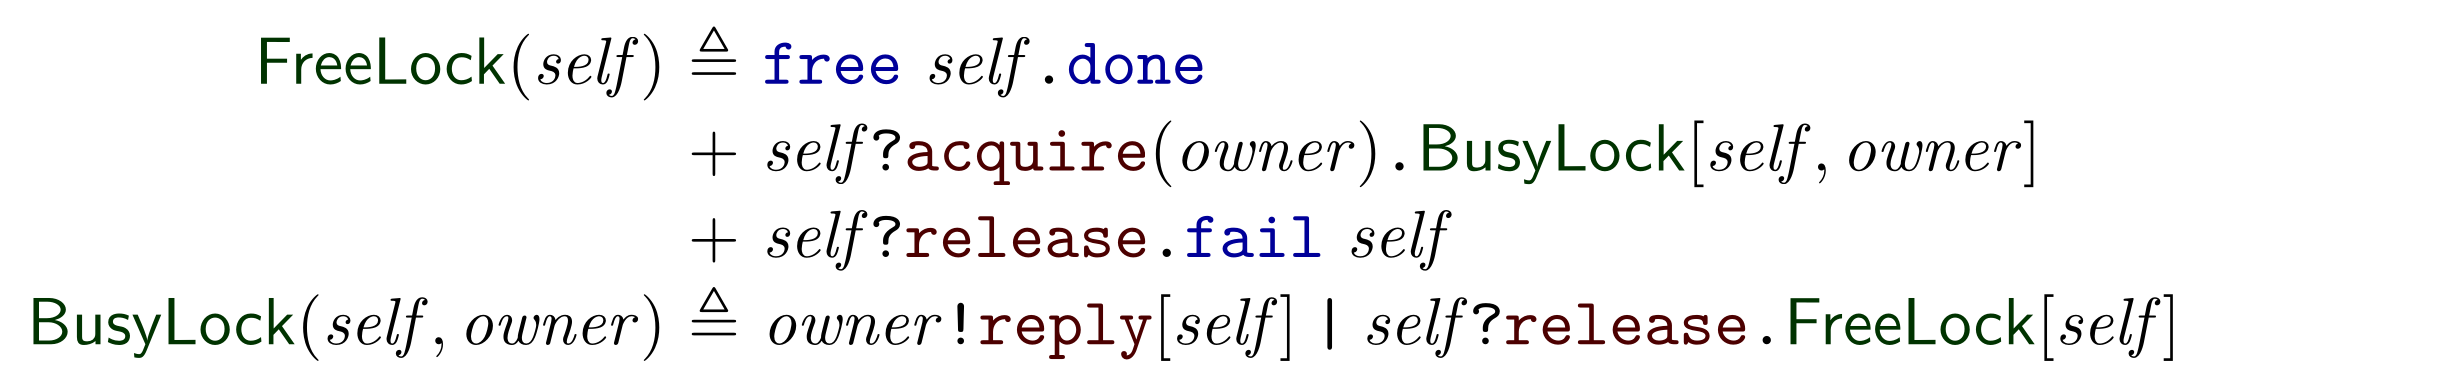
\includegraphics[width=\textwidth]{example1-lock}
    \end{figure}
    \vspace{-1em}
    \begin{figure}[H]
        \centering
        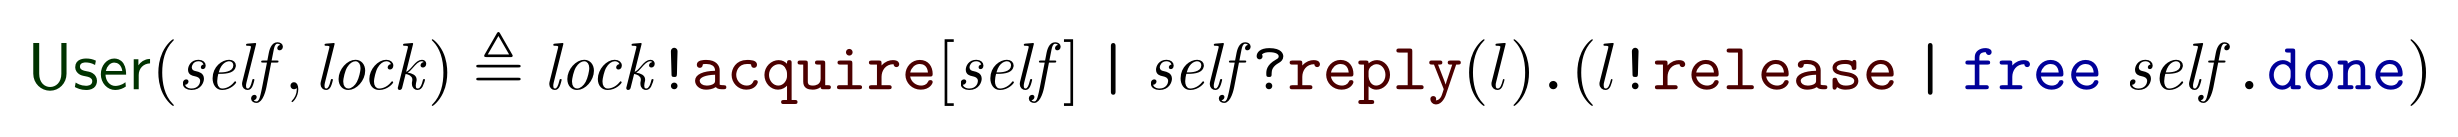
\includegraphics[width=\textwidth]{example1-user}
    \end{figure}
    \vspace{-1em}
    \begin{figure}[H]
        \centering
        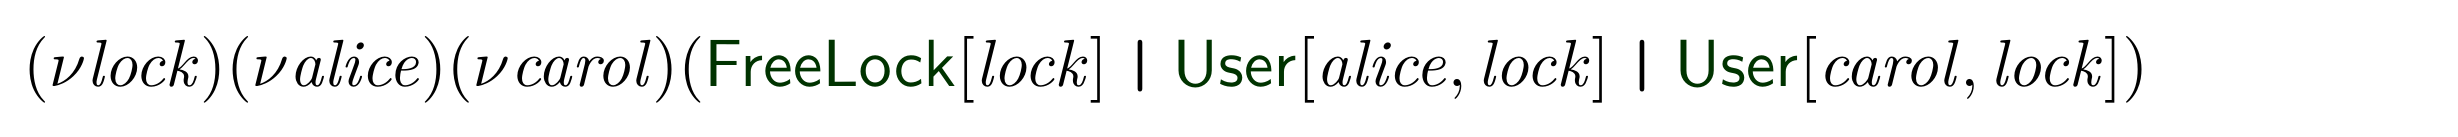
\includegraphics[width=\textwidth]{example1-usage}
    \end{figure}

    \begin{block}{Observaciones}
        \begin{itemize}
            \item \texttt{FreeLock} consume de manera no determinística los mensajes \msgtag{acquire}.
            \item \texttt{User} utiliza la referencia $l$ para enviar el mensaje \msgtag{release} ya que es ésta la referencia al mailbox que tiene la capabilidad de procesar este mensaje.
        \end{itemize}
    \end{block}
\end{frame}

\begin{frame}{Mailbox calculus}{Caracterizaciones operacionales}
    \begin{block}{Contextos de procesos}
        \vspace{-0.5em}
        \begin{figure}[H]
            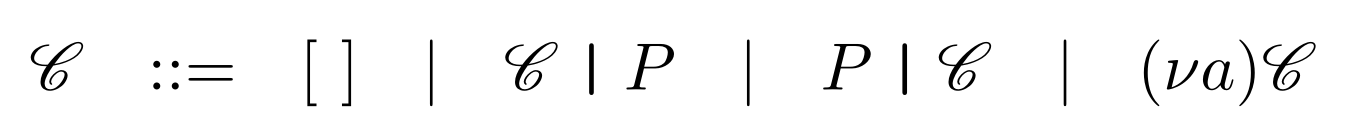
\includegraphics[width=0.7\textwidth,left]{process-context}
        \end{figure}
        \vspace{-1em}
        Los contextos de procesos buscan identificar un ``unguarded hole'', es decir un agujero que no tiene prefijada una acción sobre un mailbox.
    \end{block}
    \begin{block}{Def 4: Mailbox conformant}
        $P$ es \emph{mailbox conformant} si $P \not\rightarrow^\ast \mathscr{C}[\fail{a}]$ para todo $\mathscr{C}$ y $a$.
        \\
        En el ejemplo del lock, ser \emph{mailbox conformant} significa nunca liberar el lock antes de adquirirlo.
    \end{block}
\end{frame}

\begin{frame}{Mailbox calculus}{Caracterizaciones operacionales}
    \begin{block}{Def 5: Deadlock free}
        $P$ es \emph{deadlock free} si $P \rightarrow^\ast Q \not\rightarrow$ implica $Q \equiv \done$.
        \\
        Un proceso se considera \emph{deadlock free} si al terminar tenemos que (1) no hay subprocesos esperando un mensaje que nunca se va a producir y (2) todos los mailbox están vacíos.
    \end{block}
    \begin{block}{Def 7: Fairly terminating}
        $P$ es \emph{fairly terminating} si $P \rightarrow^\ast Q$ implica que $Q \rightarrow^\ast \done$.
        \\
        Es una propiedad más fuerte que deadlock freedom. Si un proceso es \emph{fairly terminating} entonces se garantiza \emph{junk freedom} (no quedan mensajes sin consumir en ningún mailbox).
    \end{block}
\end{frame}

\begin{frame}{Mailbox type system}{Sintaxis}
    \begin{figure}[H]
        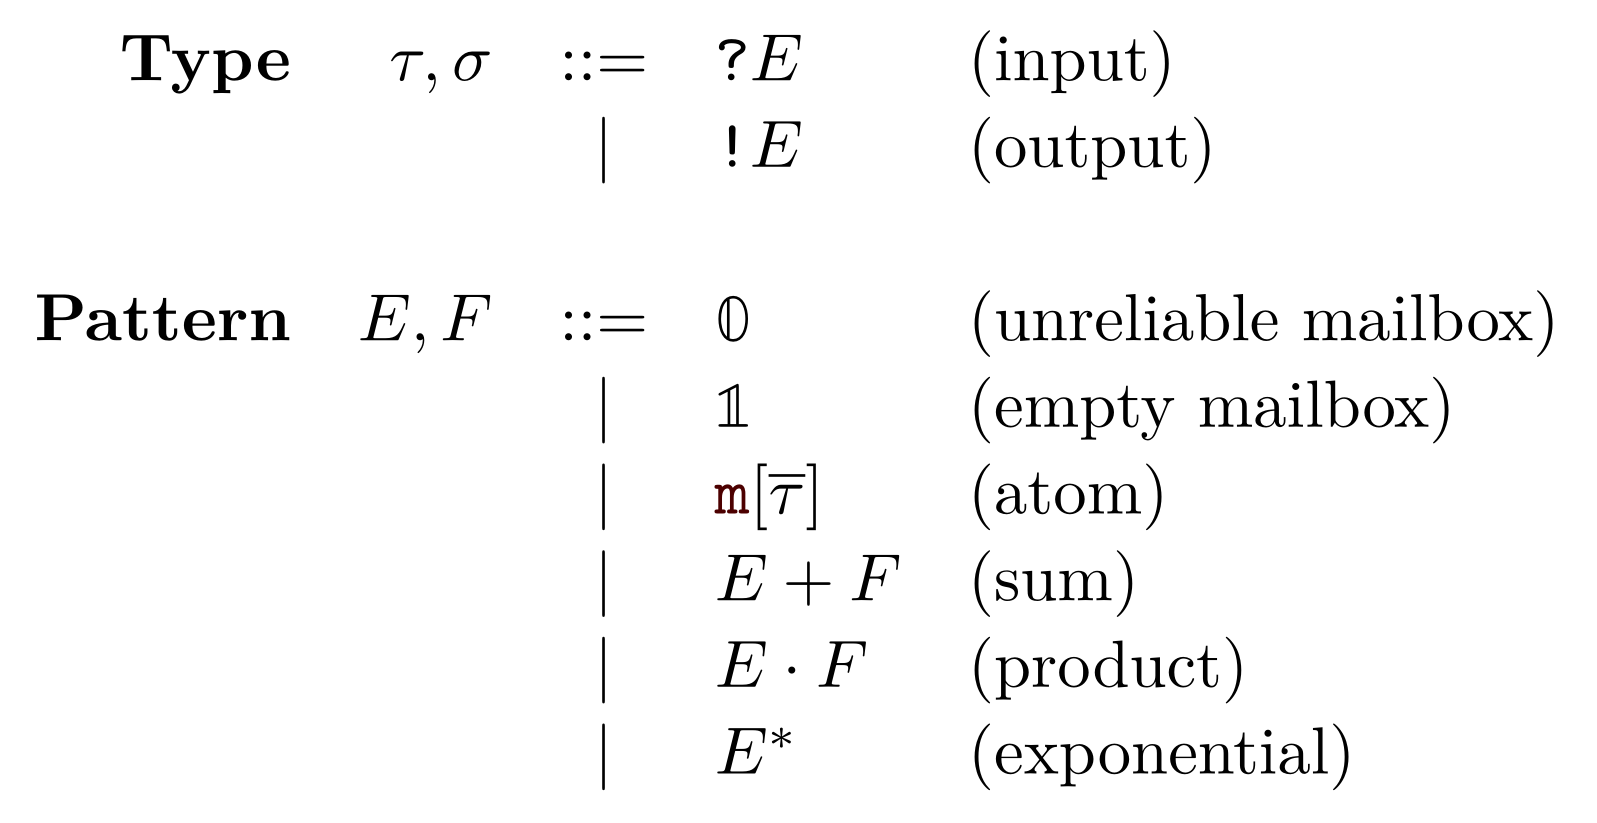
\includegraphics[width=0.9\textwidth]{type-syntax}
    \end{figure}
\end{frame}

\begin{frame}{Mailbox type system}{Patrones}
    Los patrones son \emph{expresiones regulares conmutativas} que describen las configuraciones válidas de los mensajes dentro de un mailbox.
    \vspace{1em}
    \begin{itemize}
        \item $\mathbb{0}$: \emph{unreliable mailbox} que recibió un mensaje inesperado.
        \item $\msgtag{A} + \msgtag{B}$: contiene un mensaje $\msgtag{A}$ o un mensaje $\msgtag{B}$ pero no ambos.
        \item $\msgtag{A} + \mathbb{1}$: contiene un mensaje $\msgtag{A}$ o está vacío.
        \item $\msgtag{A} \cdot \msgtag{B}$: contiene un mensaje $\msgtag{A}$ y un mensaje $\msgtag{B}$.
        \item $\msgtag{A}^\ast$: contiene un cantidad arbitraria (incluso $0$) de mensajes $\msgtag{A}$.
    \end{itemize}
\end{frame}

\begin{frame}{Mailbox type system}{Capabilities}
    Un \emph{mailbox type} consiste en un \emph{capability} ($?$ o $!$) junto a un patrón. Un proceso debe cumplir ciertas obligaciones y tiene ciertas garantías descriptas por el mailbox type asociado al mailbox que usa.
    \vspace{1em}
    \begin{itemize}
        \item $!\msgtag{A}$: el proceso \textbf{debe} escribir un mensaje $\msgtag{A}$ en el mailbox.
        \item $?\msgtag{A}$: el proceso tiene \textbf{garantizado} recibir un mensaje $\msgtag{A}$.
    \end{itemize}
\end{frame}

\begin{frame}{Mailbox type system}{Capabilities: más ejemplos}
    \vspace{1em}
    \begin{itemize}
        \item $!(\msgtag{A} + \mathbb{1})$: el proceso \textbf{puede} escribir un mensaje $\msgtag{A}$ en el mailbox, pero no está obligado a hacerlo.
        \item $!(\msgtag{A} + \msgtag{B})$: el proceso \textbf{debe} escribir un mensaje $\msgtag{A}$ o $\msgtag{B}$, pero puede \textbf{elegir} cuál.
        \item $?(\msgtag{A} + \msgtag{B})$: el proceso \textbf{debe} estar preparado para recibir tanto un mensaje $\msgtag{A}$ como $\msgtag{B}$.
        \item $?(\msgtag{A} \cdot \msgtag{B})$: el proceso tiene \textbf{garantizado} recibir un mensaje $\msgtag{A}$ y otro $\msgtag{B}$, y puede elegir en qué orden recibirlos.
        \item $!(\msgtag{A} \cdot \msgtag{B})$: el proceso \textbf{debe} escribir un mensaje $\msgtag{A}$ y otro $\msgtag{B}$.
        \item $!\msgtag{A}^\ast$: el proceso \textbf{elige} cuántos mensajes $\msgtag{A}$ escribir.
        \item $?\msgtag{A}^\ast$: el proceso \textbf{debe} estar preparado para recibir una cantidad arbitraria de mensajes $\msgtag{A}$.
    \end{itemize}
\end{frame}

\begin{frame}{Mailbox type system}{Semántica de patrones}
    La semántica de los patrones se define como conjuntos de multiconjuntos de átomos: $\msgstore{m}{\tau}$.

    \begin{figure}[H]
        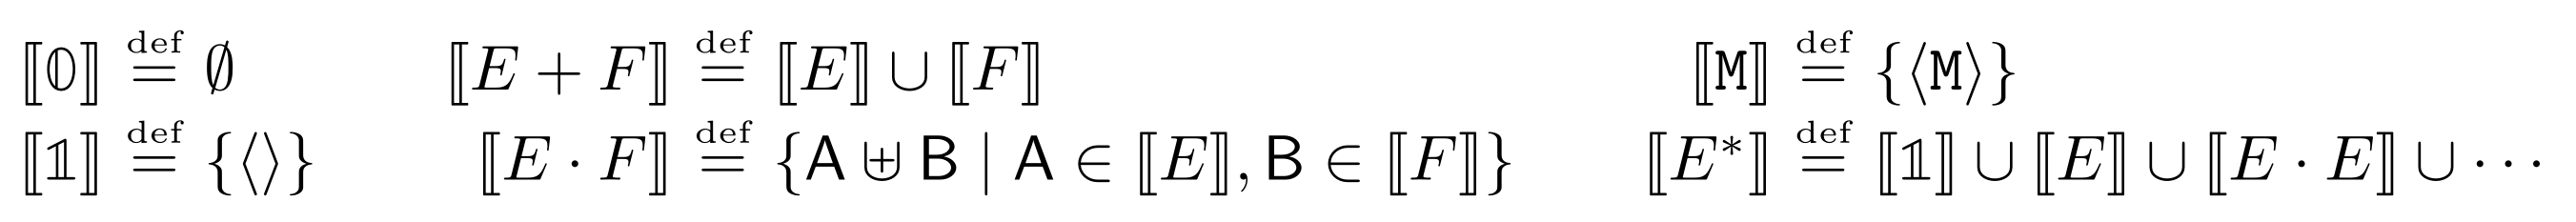
\includegraphics[width=\textwidth]{subpattern}
    \end{figure}

    Dada una relación preorder $\mathscr{R}$ sobre los tipos básicos, escribimos $E \sqsubseteq_\mathscr{R} F$ para decir que E es un subpatrón de F si $\langle \msgtag{m}_i[\overline{\tau}_i] \rangle_{i \in I} \in \llbracket E \rrbracket$ implica $\langle \msgtag{m}_i[\overline{\sigma}_i] \rangle_{i \in I} \in \llbracket F \rrbracket$ y además $\overline{\tau}_i \hspace{0.25em} \mathscr{R} \hspace{0.25em} \overline{\sigma}_i$ para todo $i \in I$.
    \vspace{1em}

    Escribimos $\simeq_\mathscr{R}$ para denotar $\sqsubseteq_\mathscr{R} \cap \sqsupseteq_\mathscr{R}$.
    \vspace{1em}

    Notemos que $\sqsubseteq_\mathscr{R}$ es covariante respecto a $\mathscr{R}$,
    \\ pues $\overline{\tau} \hspace{0.25em} \mathscr{R} \hspace{0.25em} \overline{\sigma}$ implica $\msgstore{m}{\tau} \sqsubseteq_\mathscr{R} \msgstore{m}{\sigma}$.
\end{frame}

\begin{frame}{Mailbox type system}{Subtipado}
    Decimos que $\mathscr{R}$ es una \emph{relación de subtipado} si $\tau \hspace{0.25em} \mathscr{R} \hspace{0.25em} \sigma$ implica
    \begin{enumerate}
        \item $\tau = \hspace{0.3em} ?E$ y $\sigma = \hspace{0.3em} ?F$ y $E \sqsubseteq_\mathscr{R} F$, o bien
        \item $\tau = \hspace{0.3em} !E$ y $\sigma = \hspace{0.3em} !F$ y $F \sqsubseteq_\mathscr{R} E$
    \end{enumerate}
    \vspace{1em}

    Escribimos $\leqslant$ para denotar la mayor relación de subtipado y decimos que $\tau$ es un subtipo de $\sigma$ si $\tau \leqslant \sigma$.
    \vspace{1em}

    Escribimos $\lessgtr$ para $\leqslant \cap \geqslant$, $\sqsubseteq$ para $\sqsubseteq_{\leqslant}$ y $\simeq$ para $\simeq_{\leqslant}$.
    \vspace{1em}

    Las 2 reglas se corresponden directamente con las reglas covariantes y contravariantes usuales para canales con capacidades de entrada y salida.
\end{frame}

\begin{frame}{Mailbox type system}{Subtipado: ejemplos}
    \begin{itemize}
        \item $?\msgtag{A} \leqslant \hspace{0.3em} ?(\msgtag{A} + \msgtag{B})$: un mailbox de tipo $?\msgtag{A}$ ofrece garantías más fuertes que otro de tipo $?(\msgtag{A} + \msgtag{B})$. Si un proceso sabe usar un mailbox donde pueden haber mensajes $\msgtag{A}$ o $\msgtag{B}$, también sabe usar un mailbox donde solo hay mensajes $\msgtag{A}$.
        \item $!(\msgtag{A} + \msgtag{B}) \leqslant \hspace{0.3em} !\msgtag{A}$: un mailbox de tipo $!(\msgtag{A} + \msgtag{B})$ es más permisivo que otro de tipo $!\msgtag{A}$. Si un proceso necesita un mailbox para escribir un mensaje $\msgtag{A}$, también le sirve un mailbox donde se puede escribir mensajes $\msgtag{A}$ o $\msgtag{B}$.
    \end{itemize}
\end{frame}


\begin{frame}{Mailbox type system}{Relaciones de subtipado especiales}
    Algunos mailbox types tienen patrones que están en cierta relación particular con las constantes $\mathbb{0}$ (unreliable mailbox) y $\mathbb{1}$ (empty mailbox). Estos tipos tienen la siguiente clasificación:
    \vspace{1em}

    \begin{itemize}
        \item \textbf{relevant}: si $\tau \not\leqslant \hspace{0.3em} !\mathbb{1}$ (caso contrario \emph{irrelevant})
        \\ Un mailbox \emph{relevant} debe usarse, mientras que uno \emph{irrelevant} puede descartarse. Todos los mailbox con input capability son \emph{relevantes}.
        \item \textbf{reliable}: si $\tau \not\leqslant \hspace{0.3em} ?\mathbb{0}$ (caso contrario \emph{unreliable})
        \\ Un mailbox \emph{reliable} no recibió mensajes inesperados. Todos los mailbox con output capability son \emph{reliable}.
        \item \textbf{usable}: si $!\mathbb{0} \not\leqslant \hspace{0.2em} \tau$ (caso contrario \emph{unusable})
        \\ Un mailbox \emph{usable} puede ser usado. Todos los mailbox con input capability son \emph{usable}.
    \end{itemize}
\end{frame}

\begin{frame}{Mailbox type system}{Ejemplo 11: lock type}
    \begin{figure}[H]
        \centering
        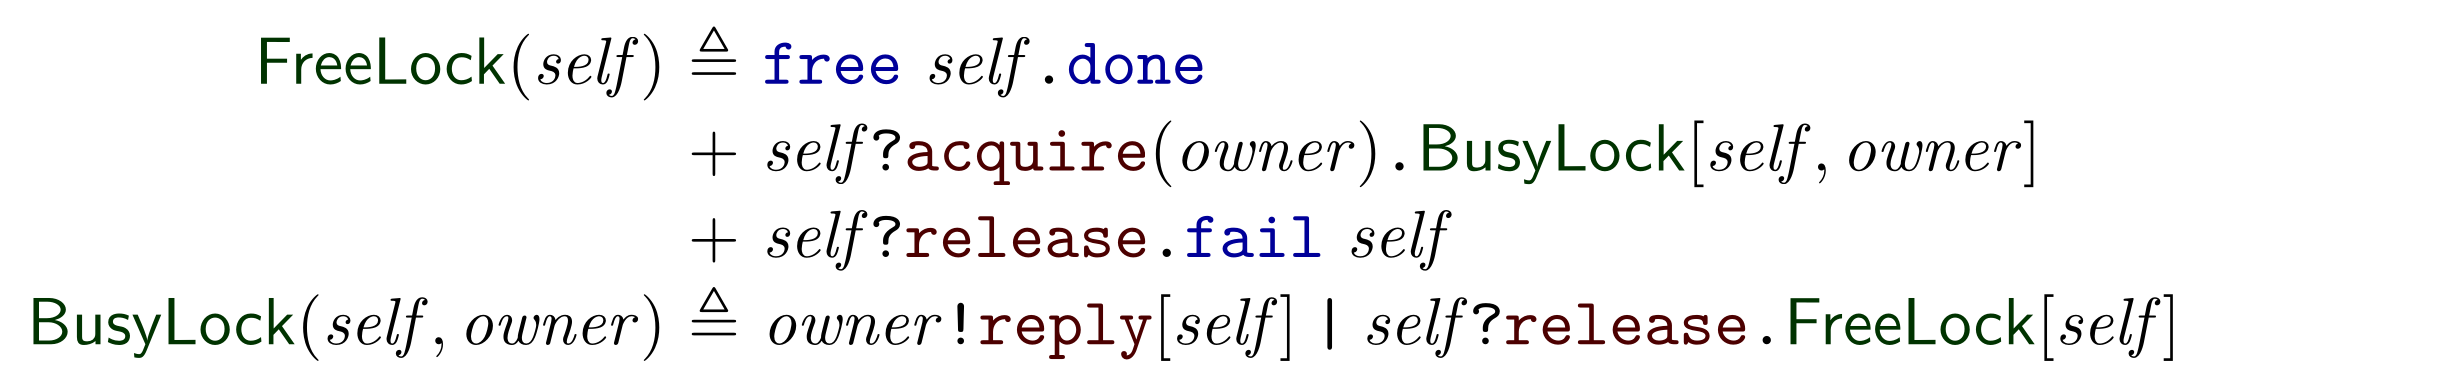
\includegraphics[width=\textwidth]{example1-lock}
    \end{figure}

    El mailbox usado por FreeLock tendrá diferentes tipos dependiendo del estado interno del lock y desde qué óptica lo miramos.
    \vspace{1em}

    \begin{itemize}
        \item Desde FreeLock: $?\msgtag{acquire}[!\msgtag{reply}[!\msgtag{release}]]^\ast$
        \item Desde BusyLock: $?(\msgtag{release} \cdot \msgtag{acquire}[!\msgtag{reply}[!\msgtag{release}]]^\ast)$
        \item Desde User hacia FreeLock: $!\msgtag{acquire}[!\msgtag{reply}[!\msgtag{release}]]^\ast$
        \item Desde Owner hacia BusyLock: $!\msgtag{release}$

    \end{itemize}
\end{frame}

\begin{frame}{Mailbox type system}{Grafo de dependencias: sintaxis}
    \begin{figure}[H]
        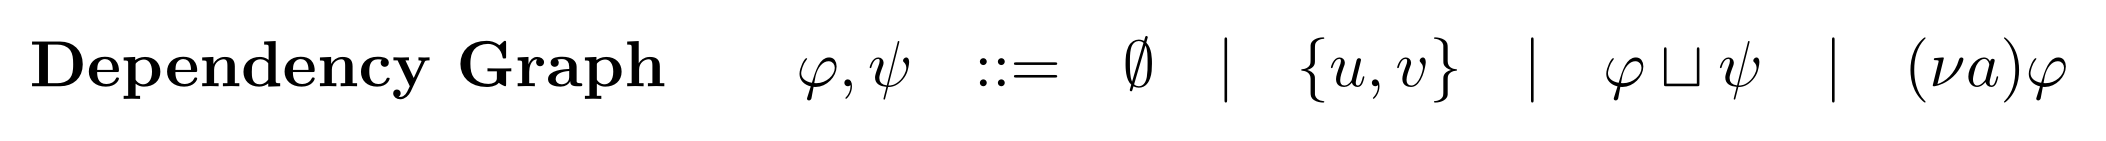
\includegraphics[width=\textwidth]{dependency-graph-syntax}
    \end{figure}

    El grafo de dependencias es un multigrafo no dirigido donde los vértices del grafo son los nombres de los mailbox y el \textbf{objetivo es trackear las dependencias entre mailboxes}. Intuitivamente hay una dependencia entre $u$ y $v$ si:
    \vspace{1em}

    \begin{itemize}
        \item $v$ es un argumento de algún mensaje del mailbox $u$,
        \item o bien $v$ aparece en la continuación de un proceso esperando un mensaje en $u$.
    \end{itemize}
\end{frame}

\begin{frame}{Mailbox type system}{Grafo de dependencias: LTS}
    \begin{figure}[H]
        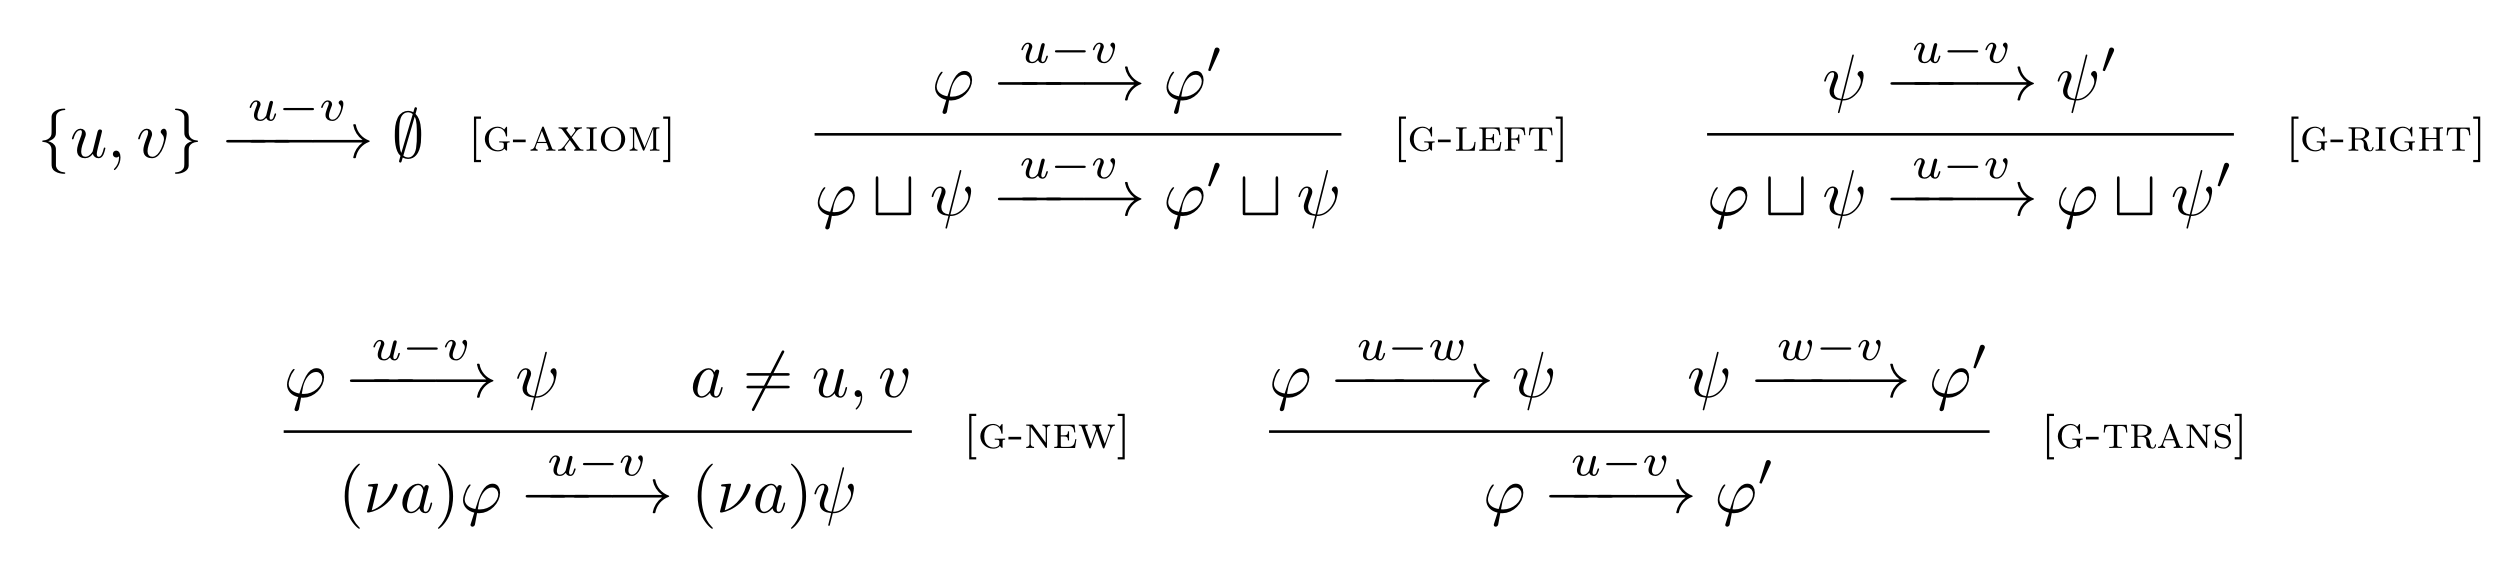
\includegraphics[width=\textwidth]{dependency-graph-lts}
    \end{figure}

    La semántica del grafo de dependencias está dada por un LTS donde el label $u - v$ representa un camino que conecta $u$ con $v$. La relación $\varphi \xrightarrow{u-v} \varphi'$ describe que $u$ está conectado con $v$ en $\varphi$, y $\varphi'$ describe el grafo residual luego de eliminar las aristas usadas para conectar $u$ con $v$.
\end{frame}

\begin{frame}{Mailbox type system}{Grafo de dependencias: propiedades}
    \begin{block}{Def 12: graph acyclicity and entailment}
        Sea $\text{dep}(\varphi) \stackrel{\text{def}}{=} \{ (u,v) \mid \exists \varphi' : \varphi \xrightarrow{u-v} \varphi' \}$ la relación de dependencias generada por $\varphi$.
        \begin{itemize}
            \item Decimos que $\varphi$ es \emph{acíclico} si $\text{dep}(\varphi)$ es irreflexiva.
            \item Decimos que $\varphi$ \emph{entails} (implica) $\psi$, escrito $\varphi \Rightarrow \psi$, si $\text{dep}(\psi) \subseteq \text{dep}(\varphi)$.
        \end{itemize}
    \end{block}
\end{frame}

\begin{frame}{Ejemplo 2: Future variable}{Definición}
    \begin{figure}[H]
        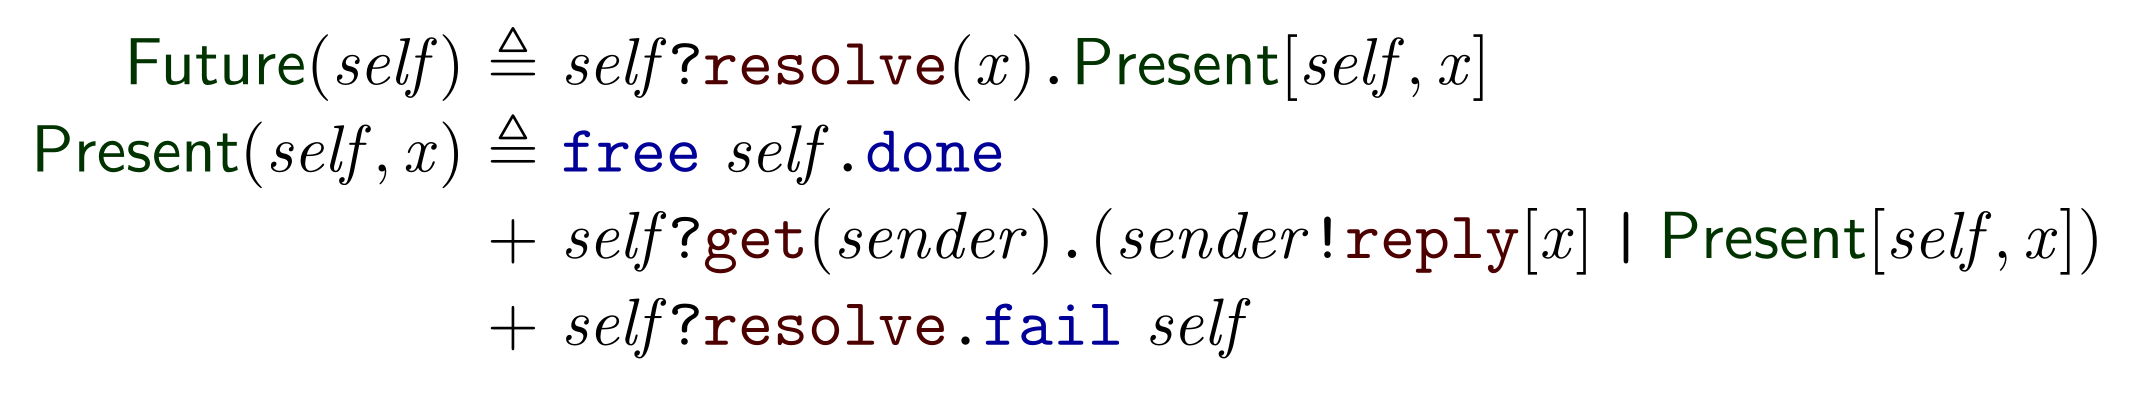
\includegraphics[width=\textwidth]{example2-future}
    \end{figure}

    \begin{itemize}
        \item Una variable futura admite un único mensaje \msgtag{put} para setear el valor de la variable.
        \item Puede recibir una cantidad arbitraria de mensajes \msgtag{get}, antes y después de ser seteada. Si se reciben antes del \msgtag{put}, estos mensajes quedan pendientes en el mailbox ya que el proceso definido por Future no tiene una guarda que selecciona los mensajes \msgtag{get}.
    \end{itemize}
\end{frame}

\begin{frame}{Ejemplo 2: Future variable}{Detección de deadlock con el grafo de dependencias}
    \begin{figure}[H]
        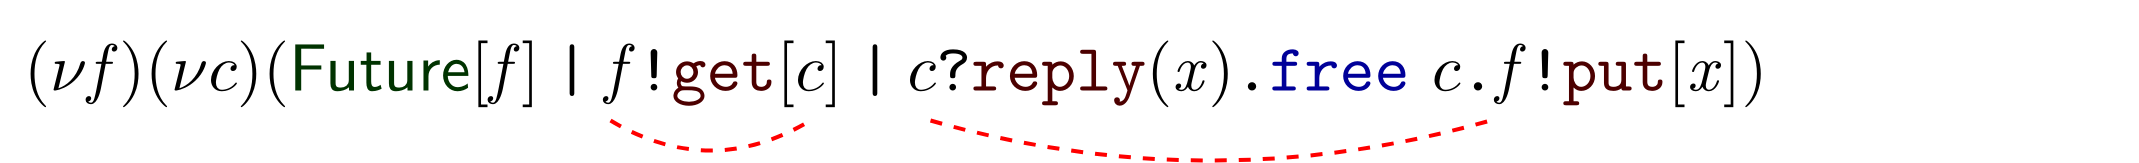
\includegraphics[width=\textwidth]{dependency-graph-example}
    \end{figure}

    \begin{itemize}
        \item El mailbox $c$ es el argumento del mensaje $\msgtag{get}$ guardado en el mailbox $f$.
        \item El mailbox $f$ aparece en la continuación luego de leer del mailbox $c$.
    \end{itemize}

    \vspace{-1em}
    \begin{figure}
        \centering
        \digraph[scale=0.5]{dependencygraph}{
            graph [rankdir=LR, pad=0.1]
            node [shape=circle, fontname="Latin Modern Mono"]
            edge [dir=none]
            f -> c
            f -> c
        }
    \end{figure}
    \vspace{-1em}

    Claramente el grafo de dependencias \textbf{tiene un ciclo}. Vamos a utilizar estos grafos en las reglas de tipado para evitar deadlocks.
\end{frame}

\begin{frame}{Mailbox type system}{Reglas de tipado}
    \begin{block}{Type environments}
        $\Gamma$ y $\Delta$ son funciones parciales de nombres a tipos: $\overline{u} : \overline{\tau}$.
    \end{block}

    \begin{block}{Procesos}
        $\Gamma \vdash P :: \varphi$
        \\
        $P$ está bien tipado bajo $\Gamma$ y genera el grafo de dependencias $\varphi$. Decimos que el juicio de tipado está bien formado si $\text{fn}(\varphi) \subseteq \text{dom}(\Gamma)$ y $\varphi$ es acíclico.
    \end{block}

    \begin{block}{Guardas}
        $\Gamma \vdash G$
    \end{block}
\end{frame}

\begin{frame}{Mailbox type system}{Reglas de tipado}
    \begin{figure}[H]
        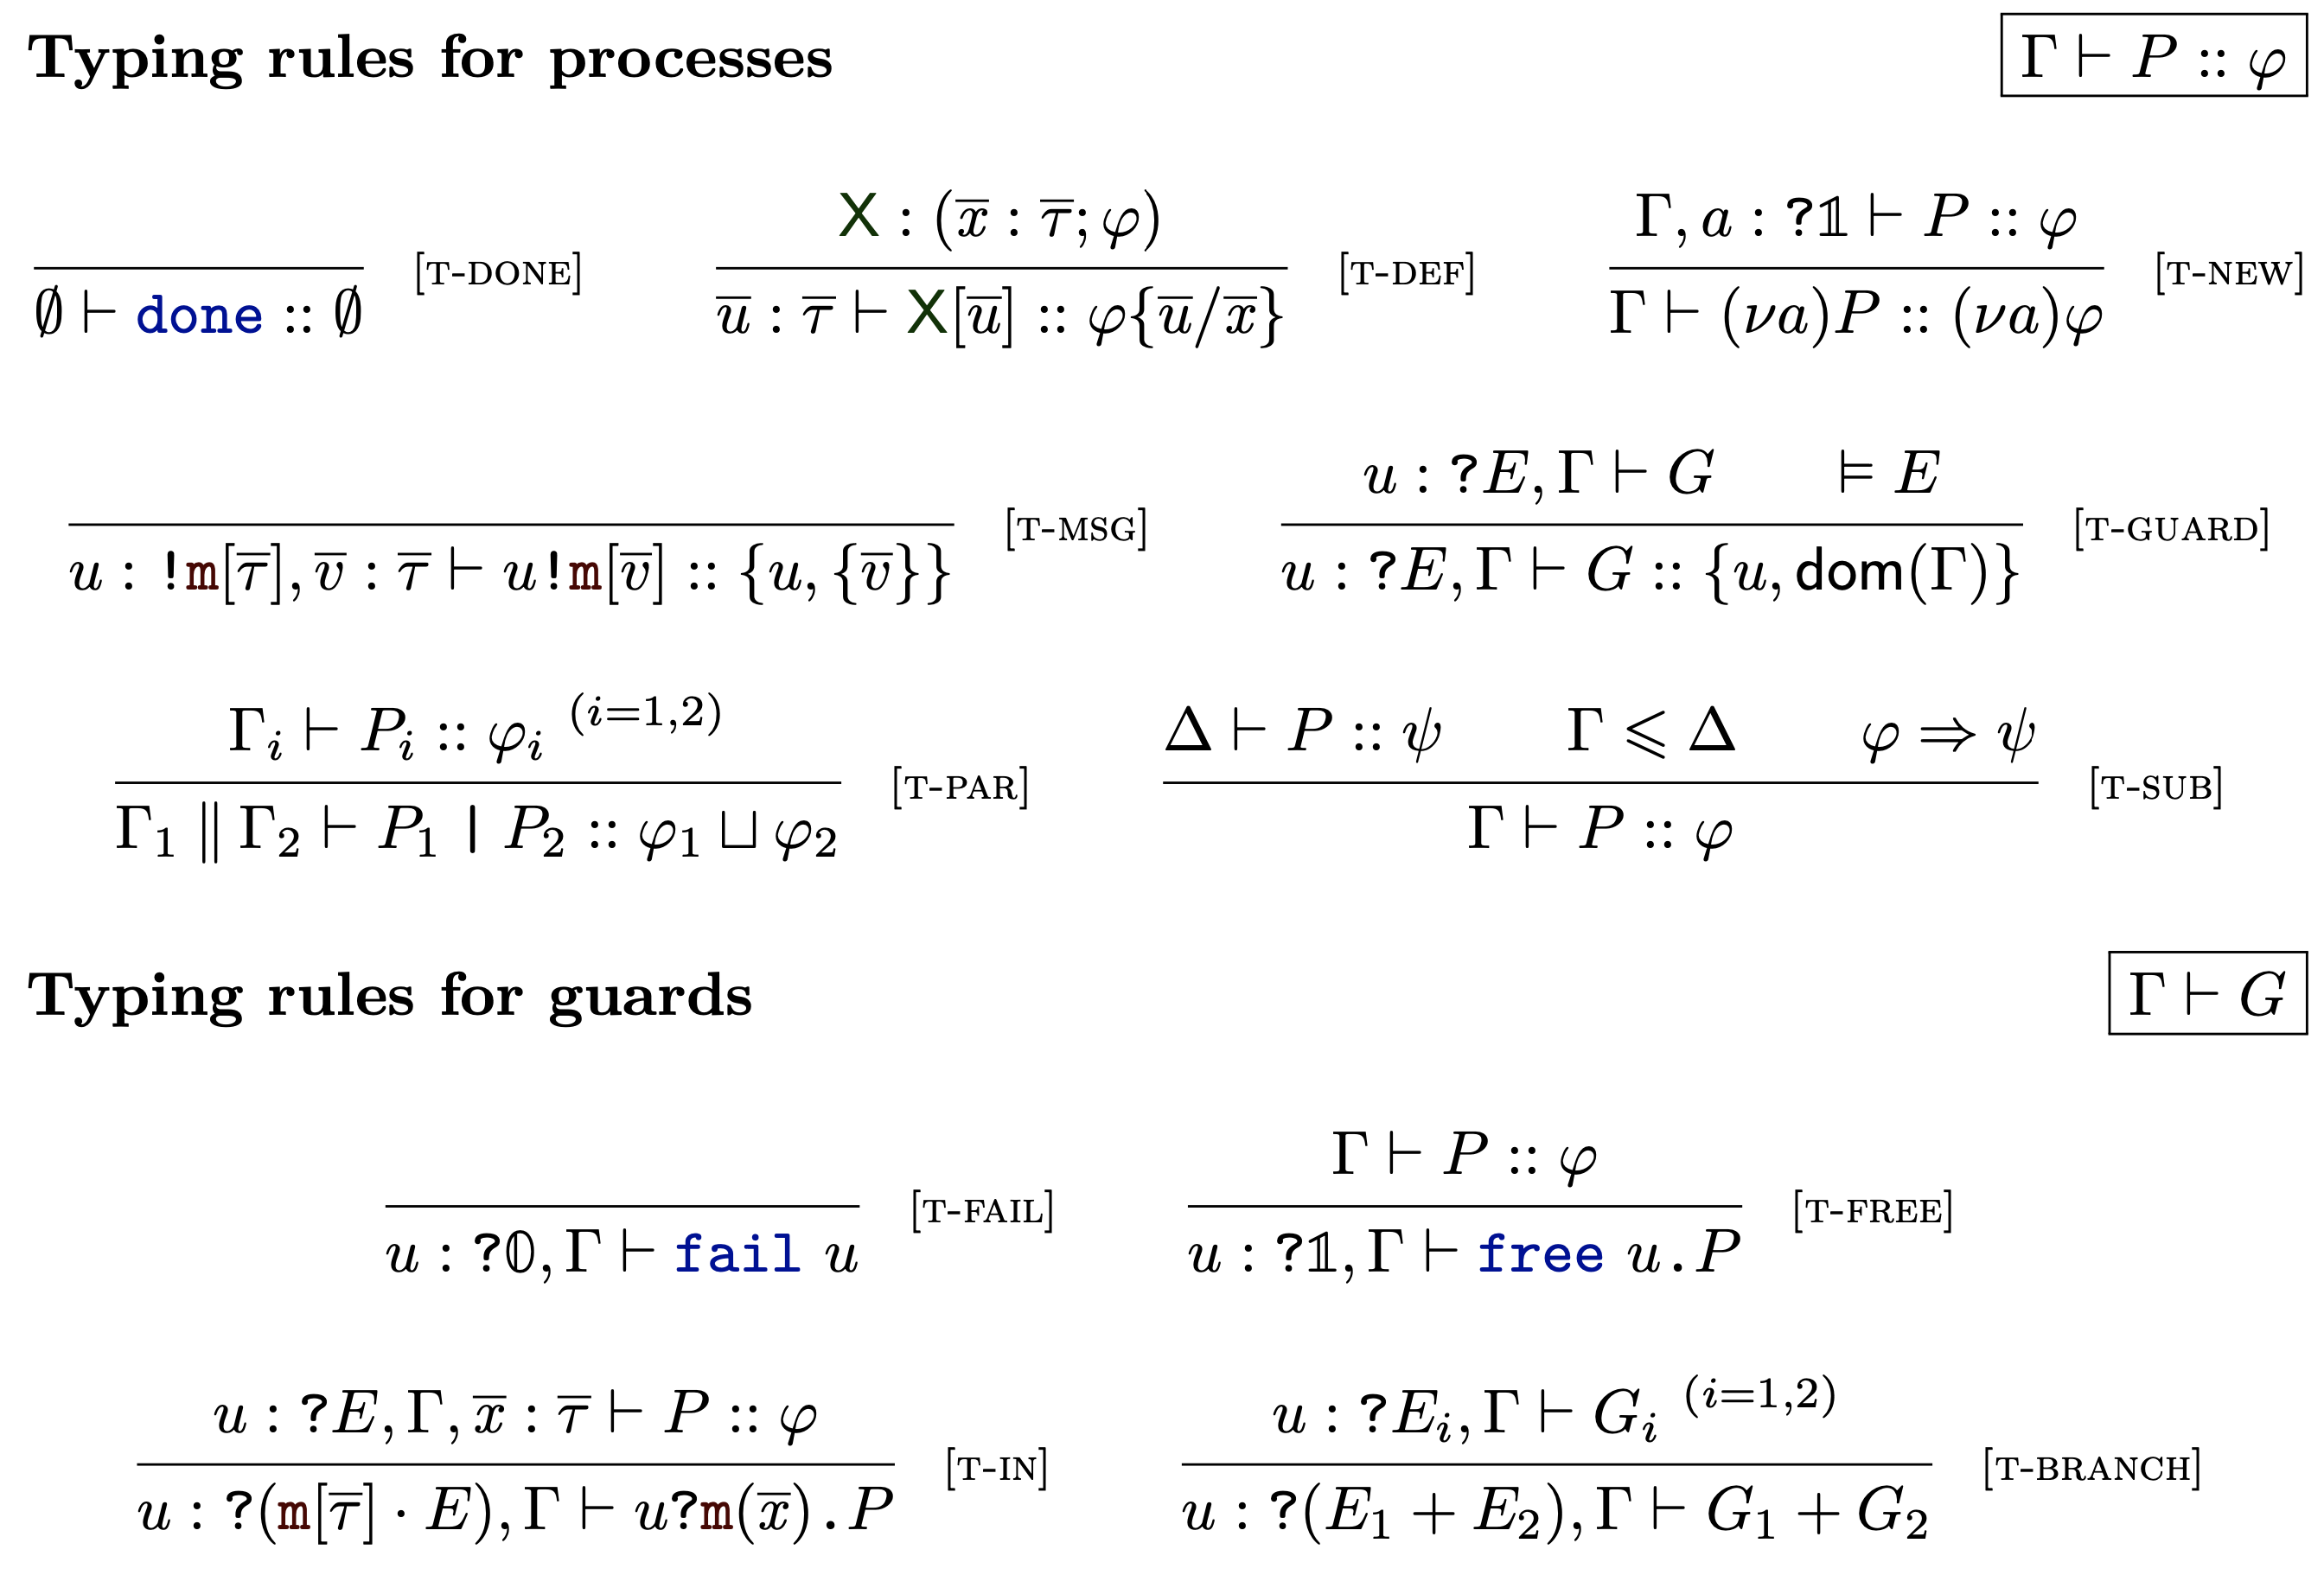
\includegraphics[width=\textwidth]{typing-rules}
    \end{figure}
\end{frame}

\begin{frame}{Mailbox type system}{\texttt{[T-MSG]}}
    \begin{figure}[H]
        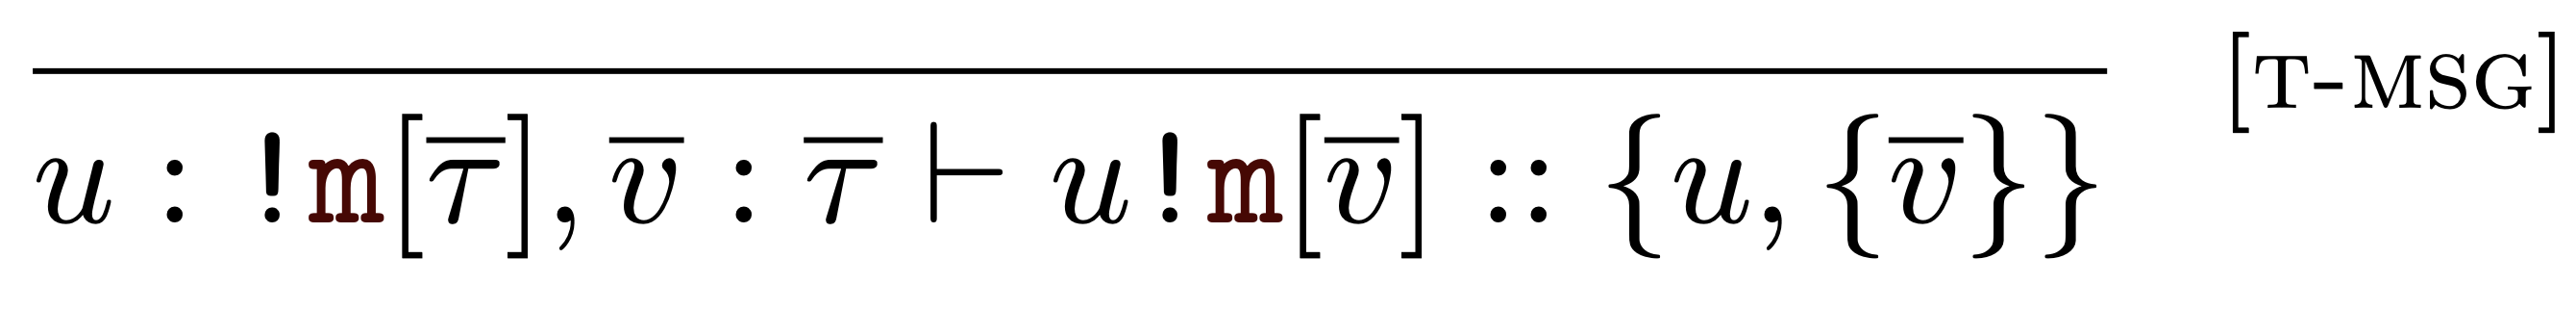
\includegraphics[height=2em]{typing-rules-t-msg}
    \end{figure}

    Un mensaje está bien tipado si el mailbox $u$ admite recibir un mensaje con tag $\msgtag{m}$ y argumentos de tipo $\overline{\tau}$, y además los valores de los argumentos $\overline{v}$ efectivamente tienen tipo $\overline{\tau}$.
    \vspace{1em}

    Enviar un mensaje genera una dependencia entre el mailbox $u$ y todos los argumentos $\overline{v}$.
    \\
    $\{ u, \{ \overline{v} \} \} \equiv \{u, v_1\} \sqcup \dots \sqcup \{u, v_n\}$
\end{frame}

\begin{frame}{Mailbox type system}{\texttt{[T-FAIL]} y \texttt{[T-FREE]}}
    \begin{figure}[H]
        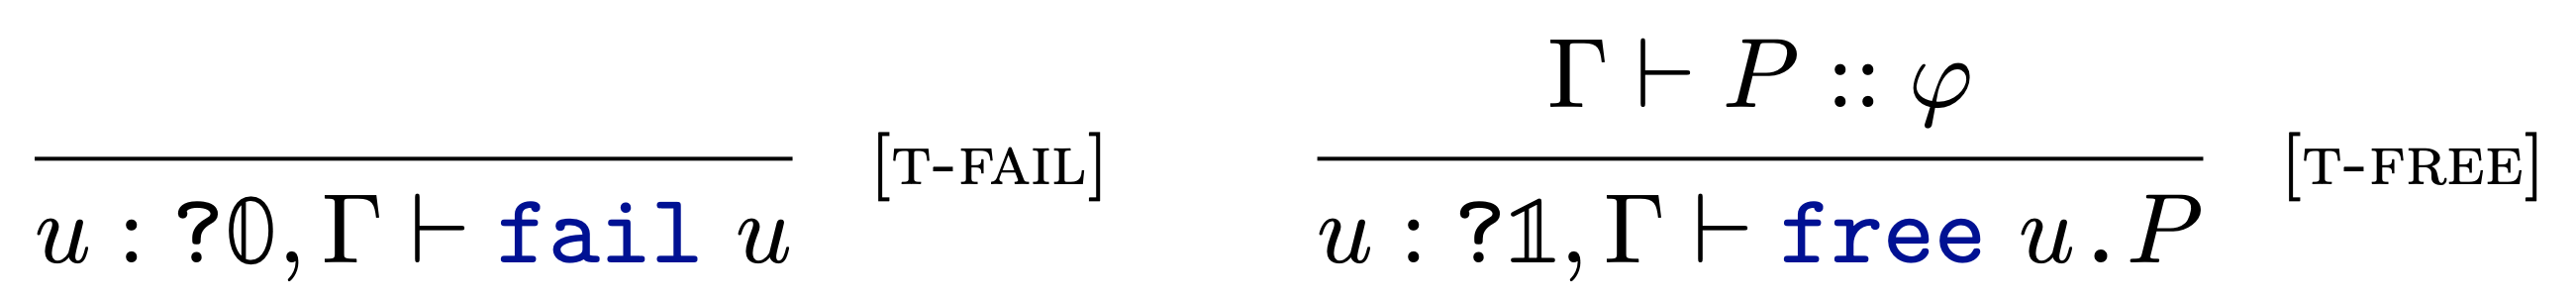
\includegraphics[height=2.5em]{typing-rules-t-fail-t-free}
    \end{figure}

    La regla \texttt{[T-FAIL]} permite tipar un \emph{runtime error} si el mailbox $u$ tiene tipo $?\mathbb{0}$ indicando que el mailbox es \emph{unreliable} (recibió un mensaje inesperado).
    \vspace{1em}

    La regla \texttt{[T-FREE]} dice que podemos liberar el mailbox $u$ si tiene tipo $?\mathbb{1}$ indicando que está vacío, siempre y cuando la continuación $P$ está bien tipada en el ambiente residual.
\end{frame}

\begin{frame}{Mailbox type system}{\texttt{[T-IN]}}
    \begin{figure}[H]
        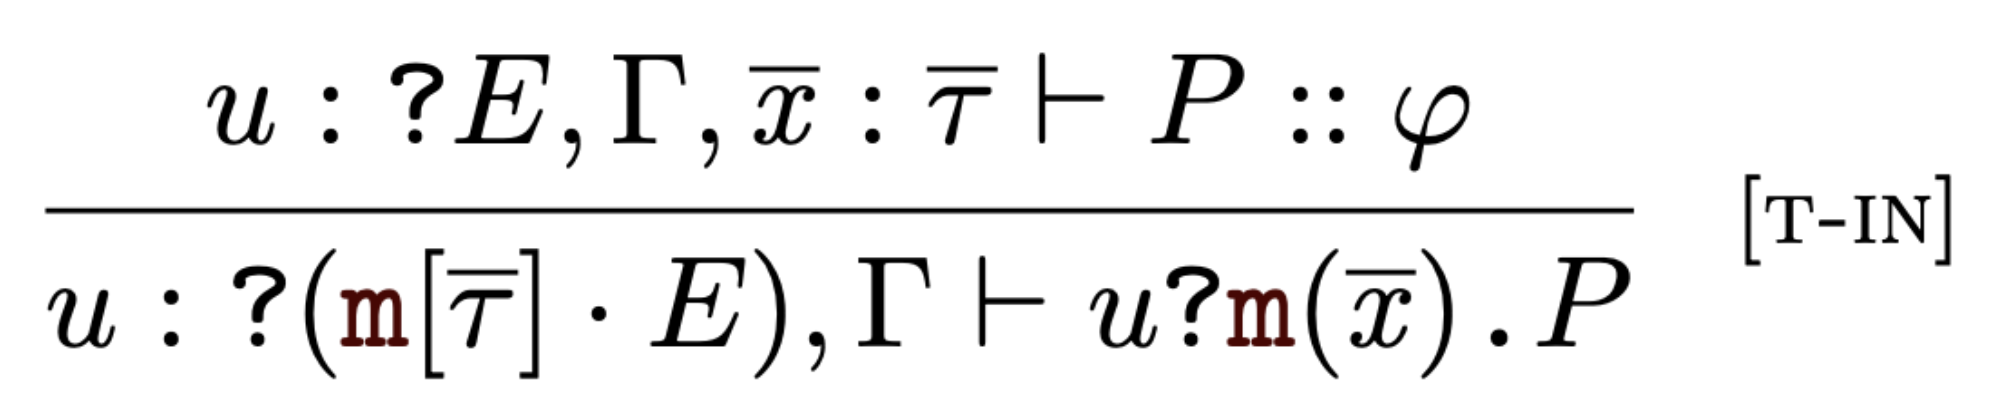
\includegraphics[height=3em]{typing-rules-t-in}
    \end{figure}

    Consumir un mensaje $\msgtag{m}$ de un mailbox $u$ requiere que el mailbox tenga tipo $?(\msgstore{m}{\tau} \cdot E)$ que garantiza que hay al menos 1 mensaje $\msgtag{m}$, posiblemente con otros mensajes acorde al patrón $E$.
    \vspace{1em}

    La continuación $P$ debe estar bien tipada en un ambiente donde el mailbox tiene tipo $?E$ que describe el contenido del mailbox luego de haber consumido el mensaje $\msgtag{m}$, y además incluye el tipo de los argumentos $\overline{x}$ del mensaje.
\end{frame}

\begin{frame}{Mailbox type system}{\texttt{[T-BRANCH]}}
    \begin{figure}[H]
        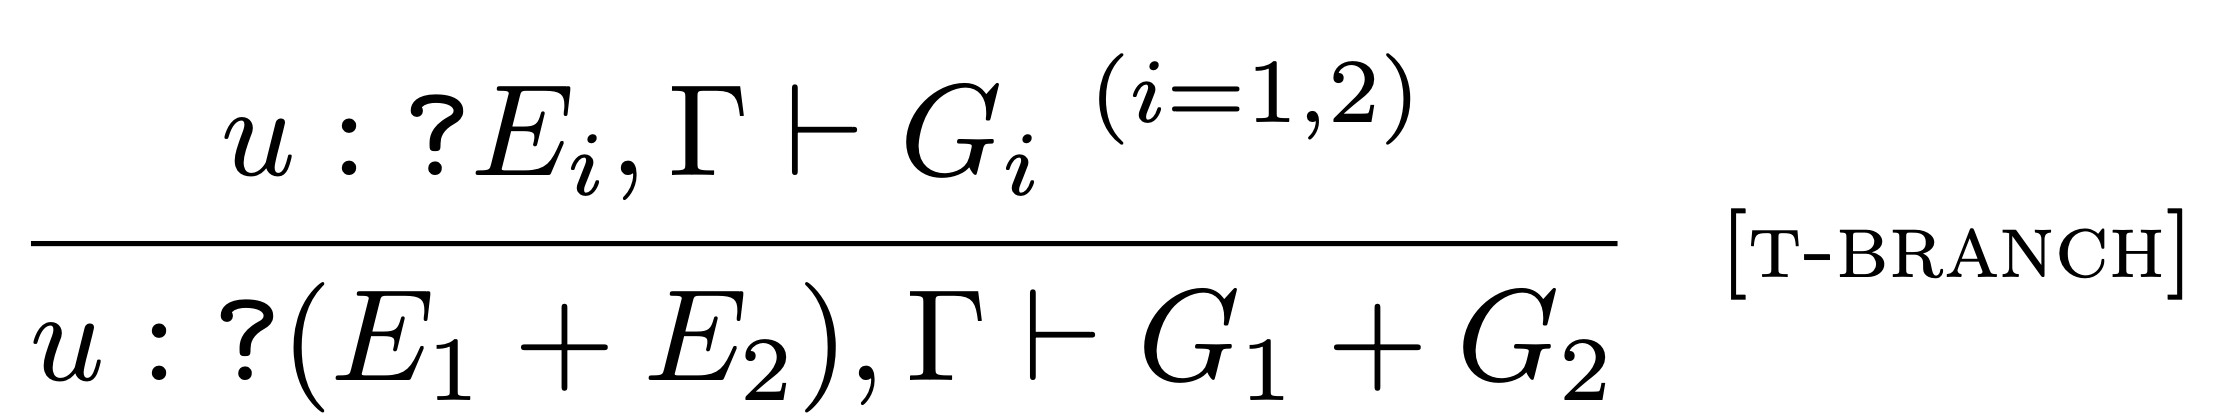
\includegraphics[height=3em]{typing-rules-t-branch}
    \end{figure}

    La composición de guardas $G_1 + G_2$ ofrece las acciones de $G_1$ y $G_2$ donde cada una se corresponde con el subpatrón $E_1$ y $E_2$ del mailbox type $?(E_1 + E_2)$.
\end{frame}

\begin{frame}{Mailbox type system}{\texttt{[T-GUARD]}}
    \begin{figure}[H]
        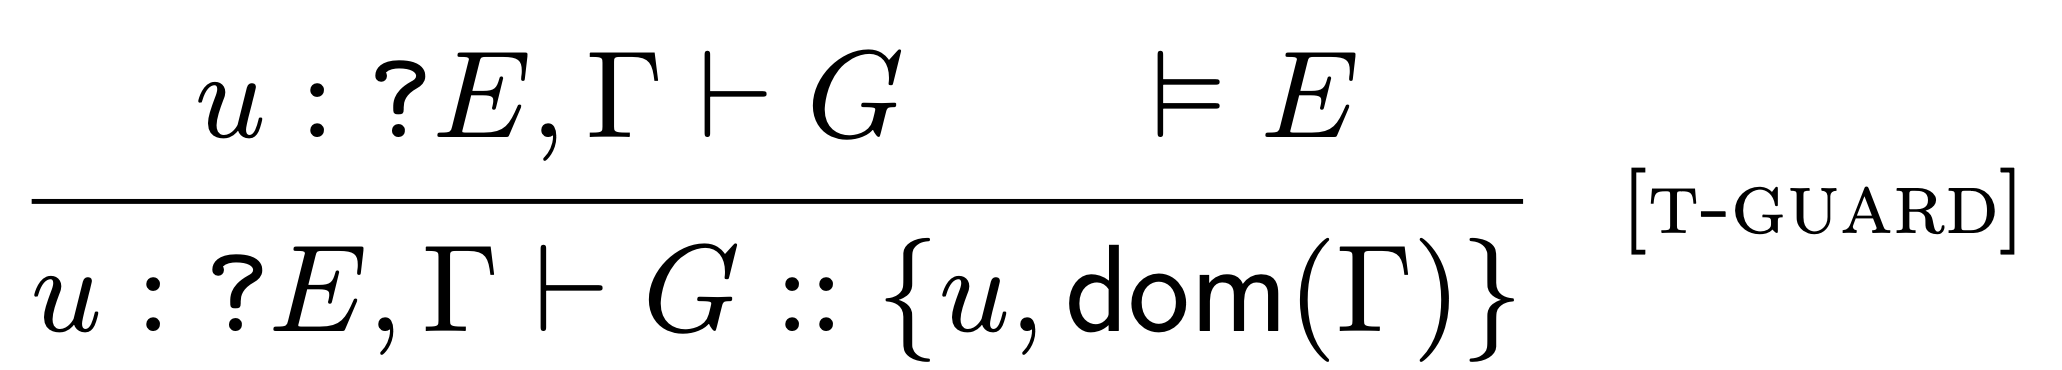
\includegraphics[height=3em]{typing-rules-t-guard}
    \end{figure}

    Esta regla tipa un \emph{guarded process} $G$ que posiblemente consume mensajes del mailbox $u$. El grafo de dependencias se define entre $u$ y todas las variables libres que aparecen en la continuación.
    \vspace{1em}

    La condición $\models E$ pide que el patrón $E$ esté en \textbf{forma normal}.
\end{frame}

\begin{frame}{Mailbox type system}{Patrones en forma normal}
    $u:?(\msgtag{A} \cdot \msgtag{C} + \msgtag{B} \cdot \msgtag{A}) \vdash u? \msgtag{A}.P + u? \msgtag{B}.Q$
    \vspace{1em}

    Si usamos la regla \texttt{[T-IN]} para tipar ambas guardas, necesitamos tipar $P$ y $Q$ en un ambiente donde el mailbox $u$ fue actualizado para reflejar que se consumió un mensaje. Podríamos inferir que para $P$ tenemos $u:?\msgtag{C}$ y para $Q$ tenemos $u:?\msgtag{A}$.
    \vspace{1em}

    Esto está mal porque el tipo de $u$ especifica que un mensaje $\msgtag{A}$ puede estar acompañado de otro mensaje $\msgtag{C}$ o $\msgtag{B}$. La solución es llevar los patrones a una \textbf{forma normal}. En este ejemplo, una forma normal podría ser: $u:?\msgtag{A} \cdot (\msgtag{B} + \msgtag{C})$.
\end{frame}

\begin{frame}{Mailbox type system}{\texttt{[T-PAR]}}
    \begin{figure}[H]
        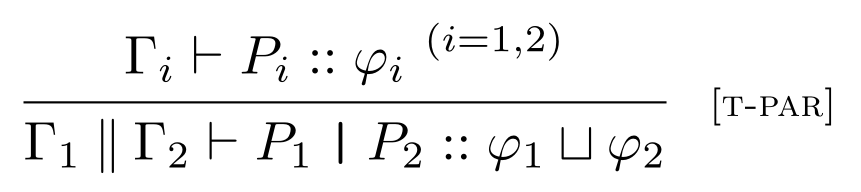
\includegraphics[height=3em]{typing-rules-t-par}
    \end{figure}

    La composición paralela $P_1 | P_2$ posiblemente necesite tipar 2 usos distintos del mismo mailbox $u$, ya que $P_1$ podría escribir un mensaje $\msgtag{A}$ en $u$ mientras que $P_2$ podría escribir otro mensaje $\msgtag{B}$. En la composición paralela $P_1 | P_2$ necesitamos tipar $u$ con un único tipo que contemple ambos mensajes.
\end{frame}

\begin{frame}{Mailbox type system}{Combinación de tipos}
    \begin{figure}[H]
        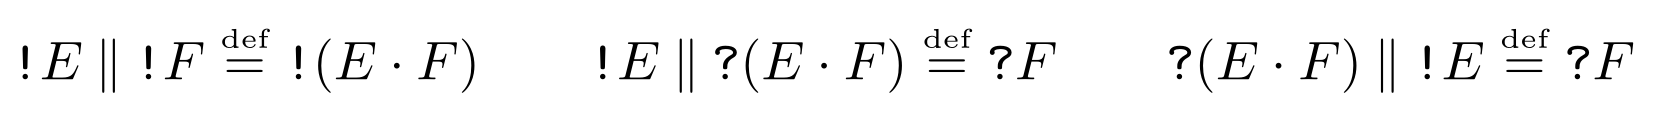
\includegraphics[width=0.9\textwidth]{type-combinator}
    \end{figure}

    \begin{itemize}
        \item $!\msgtag{A} \parallel !\msgtag{B} = !(\msgtag{A} \cdot \msgtag{B})$
            \\ Guardar un mensaje $\msgtag{A}$ y otro $\msgtag{B}$ es equivalente al patrón producto $\msgtag{A} \cdot \msgtag{B}$.
        \item $!\msgtag{A} \parallel ?(\msgtag{A} \cdot \msgtag{B}) = ?\msgtag{B}$
            \\ Cuando el mailbox se usa para input y output, el tipo combinado es el \textbf{balance final de mensajes} en el mailbox.
    \end{itemize}

    El operator $\parallel$ se extiende inductivamente para la combinación de ambientes.
\end{frame}

\begin{frame}{Mailbox type system}{\texttt{[T-NEW]}}
    \begin{figure}[H]
        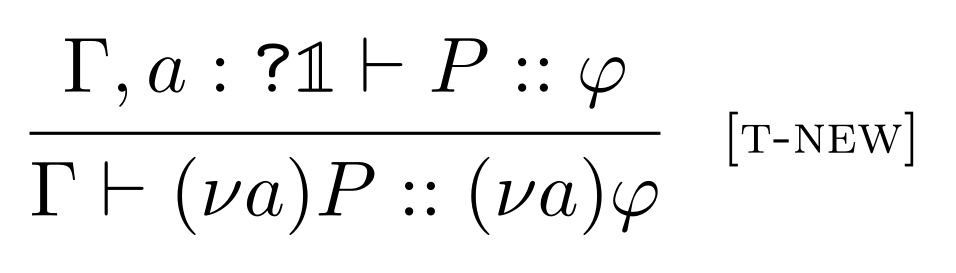
\includegraphics[height=3em]{typing-rules-t-new}
    \end{figure}

    Al crear un nuevo mailbox $a$ con scope $P$ pedimos que el tipo de $a$ sea $?\mathbb{1}$ (mailbox vacío) indicando que todos los mensajes producidos por los subprocesos de $P$ son todos eventualmente consumidos (también por subprocesos de $P$).
    \vspace{1em}

    El uso de $a$ por $P$ y sus subprocesos es \textbf{balanceado}.
\end{frame}

\begin{frame}{Propiedades de procesos bien tipados}
    \begin{block}{Teo 23: Subject reduction}
        Si $\Gamma$ es \emph{reliable}, $\Gamma \vdash P :: \varphi$ y $P \rightarrow Q$ entonces $\Gamma \vdash Q :: \varphi$
    \end{block}
    \vspace{1em}

    En contraste con otros tipos comportamentales, en particular con session types, los mailbox types usados por un proceso no cambian. Es decir no es necesario realizar una reducción de los mailbox types para preservar el tipo del proceso.
    \vspace{1em}

    Este resultado se ancla fuertemente en la idea de que el tipo del mailbox refleja el \textbf{balance} final de mensajes. La preservación de tipos garantiza que un proceso no va a consumir más mensajes de los que se producen, ni va a producir más mensajes de los que se consumen.
\end{frame}

\begin{frame}{Propiedades de procesos bien tipados}
    \begin{block}{Teo 24: Soundness (resultado principal)}
        Si $\emptyset \vdash P :: \varphi$ entonces $P$ es \emph{mailbox conformant} y \emph{deadlock free}.
    \end{block}
    \vspace{1em}

    Los procesos cerrados y bien tipados tienen la garantía de ser \emph{mailbox conformant} (no reciben mensajes inesperados) y además son \emph{deadlock free}.
\end{frame}

\begin{frame}{Propiedades de procesos bien tipados}
    \begin{block}{Teo 25: Fair termination}
        Si $\emptyset \vdash P :: \varphi$ y $P$ es \emph{finitely unfolding}
        \\ entonces $P$ es \emph{fairly terminating}.
    \end{block}
    \vspace{1em}

    Decimos que $P$ es \emph{finitely unfolding} si todas las reducciones maximales de $P$ usan \texttt{[R-DEF]} (invocación de procesos) una cantidad \textbf{finita} de veces.
    \vspace{1em}

    La intuición es que $P$ es fairly terminating si se invoca una cantidad finita de procesos. Al estar $P$ bien tipado bajo el ambiente vacío, concluimos que todos los mailboxes tienen un balance final nulo, es decir terminan vacíos, y por lo tanto se puede garantizar \emph{junk freedom} (no hay mensajes sin consumir).
\end{frame}

\begin{frame}{Fair termination}
    \begin{block}{}
        $(\nu a)(a!\msgtag{m} | \text{X}[a])$ con $\text{X}(x) \triangleq \text{X}[x]$
    \end{block}
    \vspace{1em}
\end{frame}

\begin{frame}{Encoding binary sessions}
\end{frame}

\begin{frame}{Related work}
\end{frame}

\begin{frame}{Conclusiones}
\end{frame}

\end{document}
